\documentclass[ordinary]{BMSTU-IU8}

\student{Н.В. Железцов}
\group{ИУ8-104}
\theme{
    Лабораторная работа на тему \\
    "Программные средства анализа речевого сигнала"
}

\discipline{Системы и сети передачи даных}
\supervisor{Ю.Г. Горшков}

\begin{document}
    \maketitle

    \tableofcontents % Содержание
    \structure{ВВЕДЕНИЕ}

Целью практических занятий является изучение и освоение основных процедур
записи, обработки, измерения параметров и анализа характеристик речевого
сигнала с использованием современных программных средств.

Запись фонограммы выполнена с помощью программы Praat. Параметры записи:
частота дискретизации 11,025 кГц, разрядность 16 бит, режим «моно», формат wav.
Произносилась фраза: «Железцов Никита Владимирович, двадцать шестое марта две
тысячи двадцать пятого года. А, Э, И, О, У, Ы».

При анализе речевого сигнала и построении сонограмм использовались
программы Praat, Sound Edit, WaveView.
 % Введение

    \structure{ТЕОРЕТИЧЕСКАЯ ЧАСТЬ}

На рисунке \ref{fig:fig01} представлено схематическое изображение источника
акустических колебаний речевого аппарата человека, слухового тракта и
спектрограмма речевого сигнала.

\begin{figure}
    \centering
    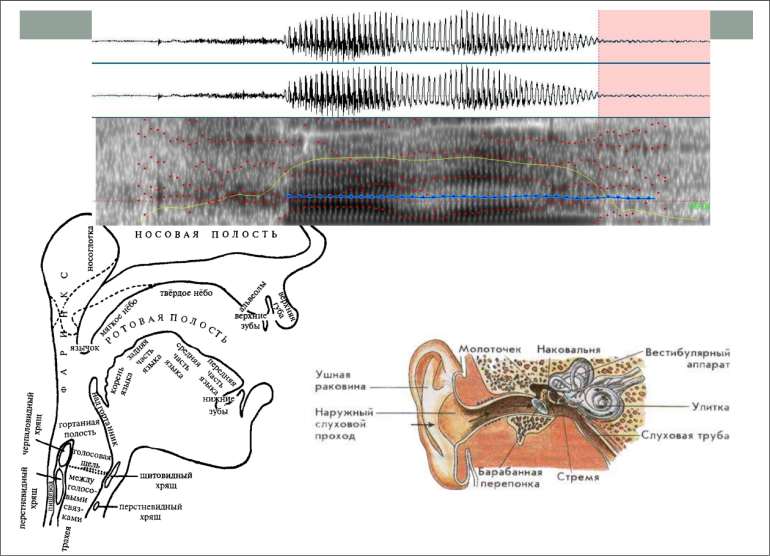
\includegraphics[scale=0.6]{inc/fig_01.png}
    \caption{
        Схематическое изображение источника акустических колебаний речевого
        аппарата человека, слухового тракта и спектрограмма речевого сигнала.
    }
    \label{fig:fig01}
\end{figure}

Речевой аппарат представляет собой неоднородную акустическую трубу, которая
изменяется по форме с течением   времени. Основными анатомическими
компонентами, вызывающими это изменение, являются губы, челюсти, язык и нёбная
занавеска (мягкое нёбо). Например, площадь сечения раскрытия губ может
изменяться от нуля (при закрытых губах) до 20 см² (при опущенной нижней челюсти
и открытых губах). Речевой тракт можно представить в виде простой модели -
линейного фильтра с изменяющимися во времени параметрами, который возбуждается
генератором периодических импульсов белого шума или их совокупности.
Анатомически линейный фильтр формируется акустической трубой, состоящей из
дыхательного (легкие, бронхи, трахея) и произносительного аппаратов (гортань с
голосовыми связками, глотка, носовая и ротовая полости, язык, нёбо, губы).


При разговоре грудная клетка расширяется и сжимается, прокачивая воздух из
лёгких по трахее через голосовую щель. Звуки образуются при выдохе воздуха при
условии, что давление воздуха под голосовыми связками превышает давление над
ними, тогда воздух, проходя через голосовую щель, смыкает и размыкает голосовые
связки, колебания которых модулируют звуковую волну.

Частота смыкания-размыкания связок представляет собой частоту основного тона
речи. Если голосовые связки расслаблены, воздух свободно проходит через
голосовую щель, не подвергаясь модуляции, и речь получается неозвученная. После
голосовых связок воздушный поток проходит через глоточную полость мимо
основания языка и, в зависимости от положения мягкого нёба, через ротовую и
(или) носовую полости, производя при этом шум.  В пространство поток воздуха
излучается в виде акустических волн и, достигнув слухового аппарата человека,
интерпретируется им как речь. Голосовой тракт (и соответствующий ему в модели
речеобразования линейный фильтр) имеет несколько резонансных областей,
создающих энергетически сильные спектральные области - форманты.

Индивидуальные акустические параметры человека определяются уникальными формой
и размерами голосового тракта, свойствами его стенок, динамикой изменения его
геометрии, формой и периодичностью импульсов голосового источника, а также
зависят от взаимодействия носовой и ротовой полостей, анатомических свойств
груди, бронхов, пазух черепа.

Характер изменения формы артикуляторов обусловлен сокращением мышц, управляемых
центральной и периферической нервными системами, которые даже у близнецов,
идеально похожих друг на друга, различаются настолько, что позволяют точно
отличить их друг от друга.

Во время произнесения неназальных звуков нёбная занавеска поднята и отделяет
голосовой тракт от носовой (назальной) полости. Носовая полость представляет
собой дополнительную акустическую трубку Эля передачи звуков, которая
используется при произнесении назальных звуков английского языка $\slash n
\slash$, $\slash m \slash$, $\slash \eta \slash$, например, в словах run, rum,
rung.

Невокализованные звуки, как, например, /f/ в слове fish, произносятся при
ненатянутых голосовых связках путём пропускания через них воздуха, причём
артикулярные органы определяют форму акустической трубы (например, путём
расположения верхних зубов на нижней губе при произнесении слова fish). При
сжатии акустической трубы и колебаниях голосовых связок произносятся
вокализованные фрикативные звуки, такие, например, как /v/ в слове van.
Взрывные звуки (например, /p/, в слове pop) произносятся путём создания
избыточного воздушного давления в области рта с последующим резким спадом после
его раскрытия.


 % Теоретическая часть
    \structure{ПРАКТИЧЕСКАЯ ЧАСТЬ}

Параметры записи: частота дискретизации 11,025 кГц, разрядность 16 бит, режим
«моно», формат wav. Произносилась фраза: «Железцов Никита Владимирович,
двадцать шестое марта две тысячи двадцать пятого года. А, Э, И, О, У, Ы ». При
анализе речевого сигнала использовано программное обеспечение: Praat, Sound
Edit, WaveView.

\subsection*{Характеристики микрофона}

За последние несколько лет наряду с аналоговыми микрофонами все большее
применение находят цифровые микрофоны. Получение высококачественных
аудиозаписей в различной акустической обстановке обеспечивают цифровые
микрофоны, например Logitech USB Desktop Microphone (рис. \ref{fig:fig02}). По
данным компании разработчика, в микрофоне используется технология подавления
шумов, позволяющая отфильтровывать фоновые шумы, в частности сигналы «фона»
сети питания 50 Гц.

\begin{figure}
    \centering
    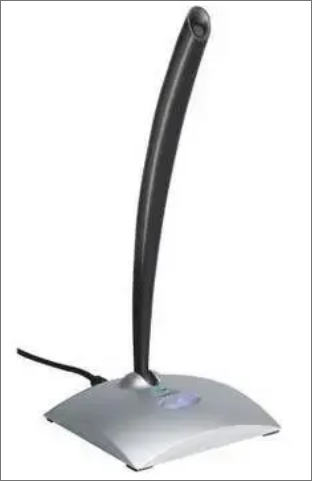
\includegraphics[scale=0.6]{inc/fig_02.png}
    \caption{ Внешний вид микрофона Logitech USB Desktop Microphone }
    \label{fig:fig02}
\end{figure}

Технические характеристики микрофона Logitech USB Desktop Microphone:

\begin{itemize}
    \item Разъем, тип А -USB
    \item Частотный диапазон, кГц - 100–16 000
    \item Чувствительность, дБ - 67
    \item Поддержка ОС - Windows 98 и старше, МаcOS 9.0.4 и старше
    \item Масса, кг - 0,392
\end{itemize}

\subsection*{Программа для анализа речи Praat}

Записанный материал был загружен в программу Praat. Перед проведением анализа
было выполнено конфигурирование приложения следующим образом. Характеристики
отображения Фурье-спектрограммы (англ. Spectrogram settings) представлены в
таблице 1.  Настройки показа формант (англ. Formants settings) - в таблице 2.
Параметры отображения траектории основного тона в координатах частота-время
(англ. Pitch settings) - в таблице 3.

\begin{table}[H]
\centering
\label{tab:tab01}
\caption{Настройки отображения Фурье-спектрограммы (Spectrogram settings)}
\begin{tabular}{|l|l|}
\hline
Параметр      & Значение        \\
\hline
View range    & 0--5000~Hz      \\
Window length & 0.005~s         \\
Dynamic range & 70.0~dB         \\
\hline
\end{tabular}
\end{table}

\begin{table}[H]
\centering
\label{tab:tab02}
\caption{Настройки показа формант (Formants settings)}
\begin{tabular}{|l|l|}
\hline
Параметр           & Значение      \\
\hline
Formant ceiling    & 5500~Hz       \\
Number of formants & 2             \\
Window length      & 0.04~s        \\
Dynamic range      & 24.0~dB       \\
Dot size           & 2.0~mm        \\
\hline
\end{tabular}
\end{table}

\begin{table}[H]
\centering
\label{tab:tab03}
\caption{Параметры отображения траектории основного тона (Pitch settings)}
\begin{tabular}{|l|l|}
\hline
Параметр     & Значение              \\
\hline
Pitch range  & 100--400.0~Hz         \\
Unit         & Hertz (логарифмический) \\
\hline
\end{tabular}
\end{table}

На рисунке \ref{fig:fig03} приведена Фурье-спектрограмма всей произнесённой
фразы, отмечена траектория основного тона в координатах
частота-время. Желтым цветом на рисунке \ref{fig:fig03} обозначена
интенсивность (intensity), синим цветом обозначена высота тона звука (pitch),
красным цветом обозначены форманты (formants).

\begin{figure}
    \centering
    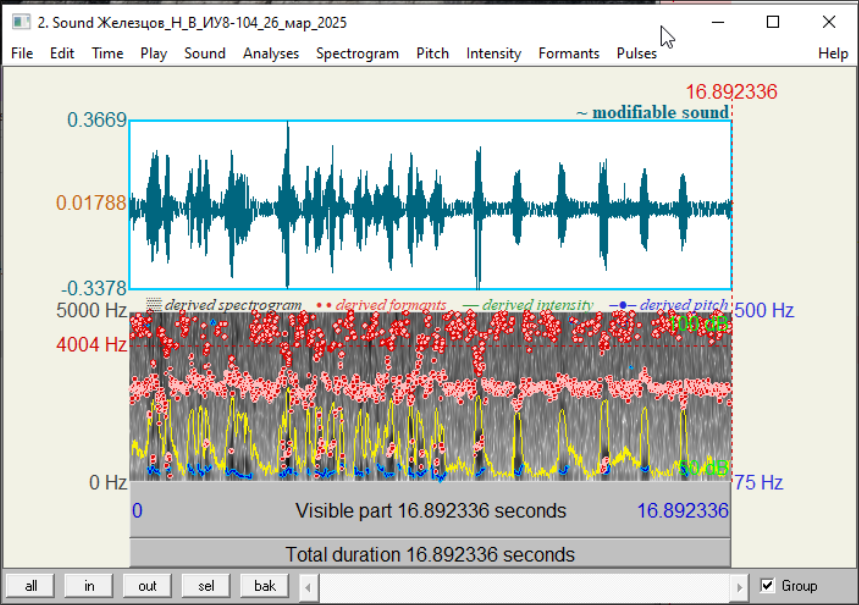
\includegraphics[scale=0.4]{inc/fig_03.png}
    \caption{
        Спектрограмма фразы «Железцов Никита Владимирович, двадцать шестое
        марта две тысячи двадцать пятого года. А, Э, И, О, У, Ы»
    }
    \label{fig:fig03}
\end{figure}

\subsection*{Звуковой редактор Sound Edit}

На рисунке \ref{fig:fig04} показана тестовая запись, а на рисунке
\ref{fig:fig05} показана Фурье-спектрограмма для тестовой записи, полученная с
использованием Sound Edit. На рисунке \ref{fig:fig06} – Вейвлет-сонограмма. На
рисунке \ref{fig:fig07} приведена Вейвлет-сонограмма для выделенных гласных
звуков «А, Э, И, О, У, Ы». Для отдельно выделенного звука «А» приведена
Фурье-спектрограмма и Вейвлет-сонограмма на рисунке \ref{fig:fig08}. Также
проанализирован спектр звука «А» с параметрами БПФ 512 и окном Блэкмана –
рисунок \ref{fig:fig09}.

\begin{figure}
    \centering
    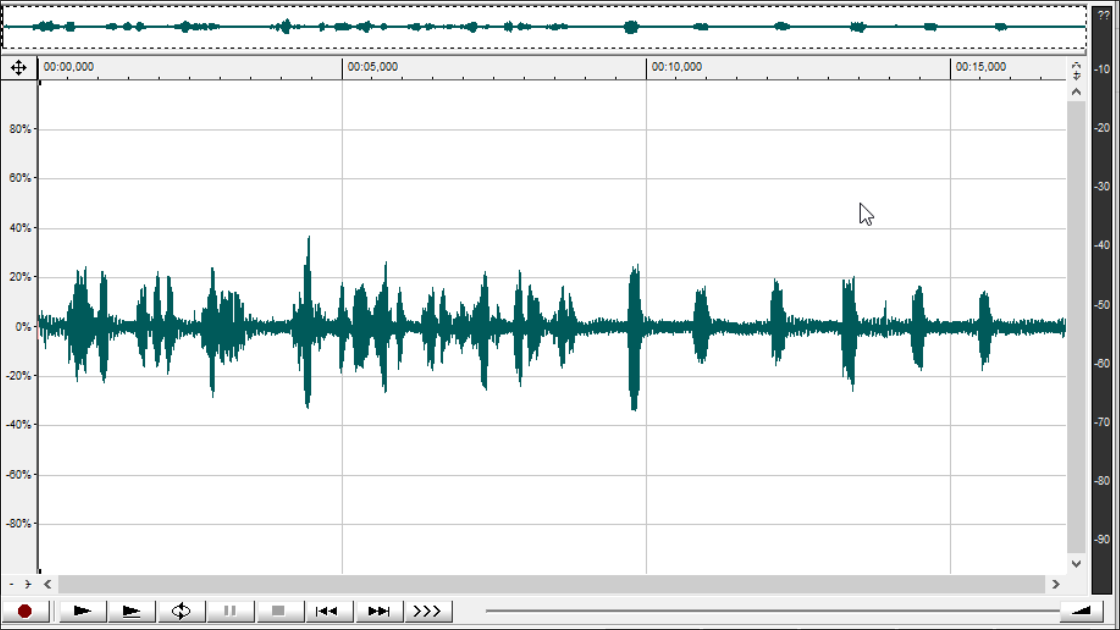
\includegraphics[scale=0.4]{inc/fig_04.png}
    \caption{Амплитуда тестовой записи в SoundEdit}
    \label{fig:fig04}
\end{figure}

\begin{figure}
    \centering
    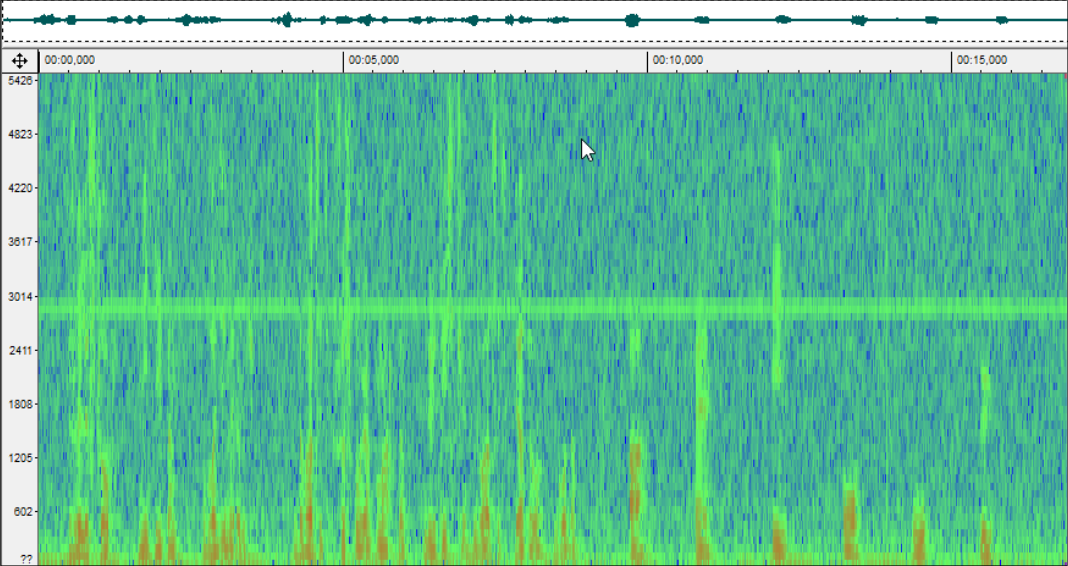
\includegraphics[scale=0.4]{inc/fig_05.png}
    \caption{Фурье-сонограмма тестовой записи в SoundEdit}
    \label{fig:fig05}
\end{figure}

\begin{figure}
    \centering
    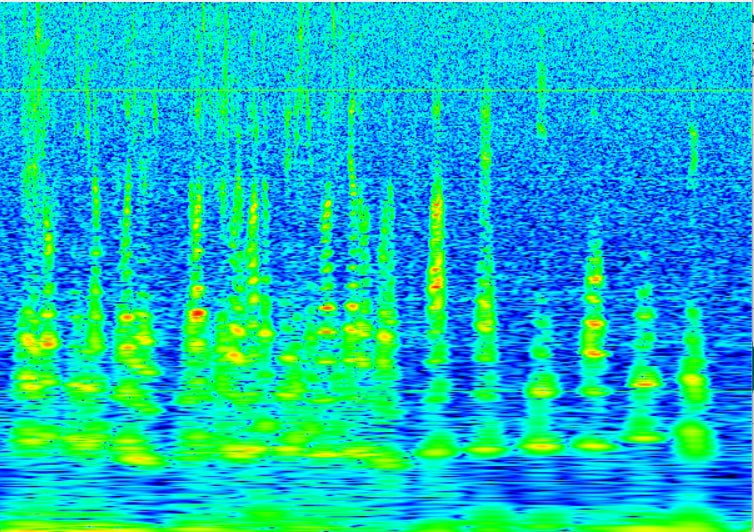
\includegraphics[scale=0.7]{inc/fig_06.jpg}
    \caption{Вейвлет-сонограмма тестовой записи в SoundEdit}
    \label{fig:fig06}
\end{figure}

\begin{figure}
    \centering
    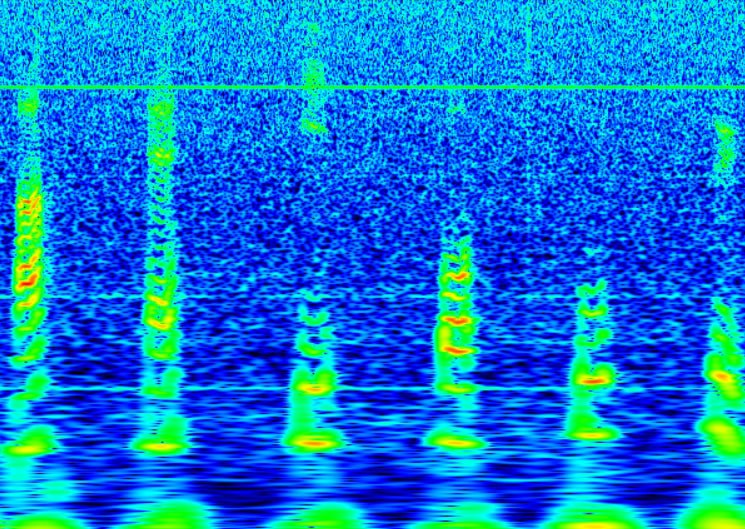
\includegraphics[scale=0.7]{inc/fig_07.jpg}
    \caption{Вейвлет-сонограмма гласных звуков «А, Э, И, О, У, Ы»}
    \label{fig:fig07}
\end{figure}

\begin{figure}
    \centering
    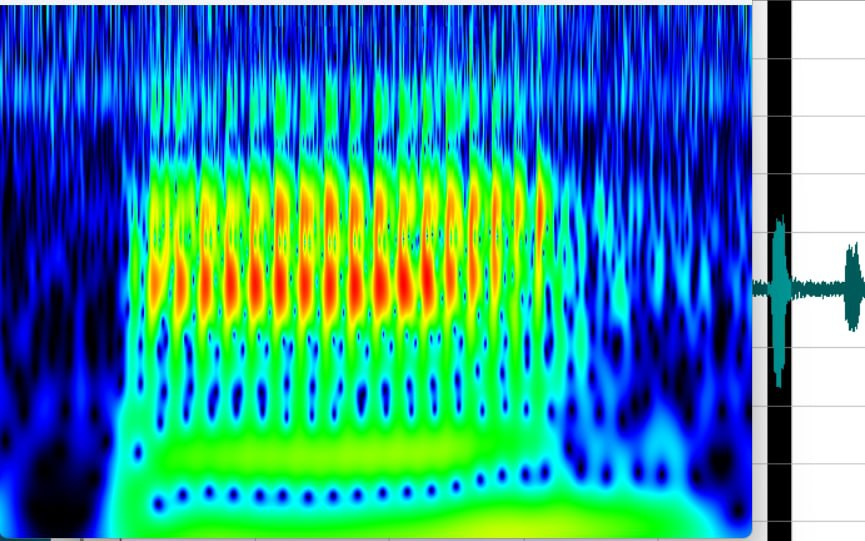
\includegraphics[scale=0.7]{inc/fig_08.jpg}
    \caption{Вейвлет-сонограмма гласного звука «А»}
    \label{fig:fig08}
\end{figure}

\begin{figure}
    \centering
    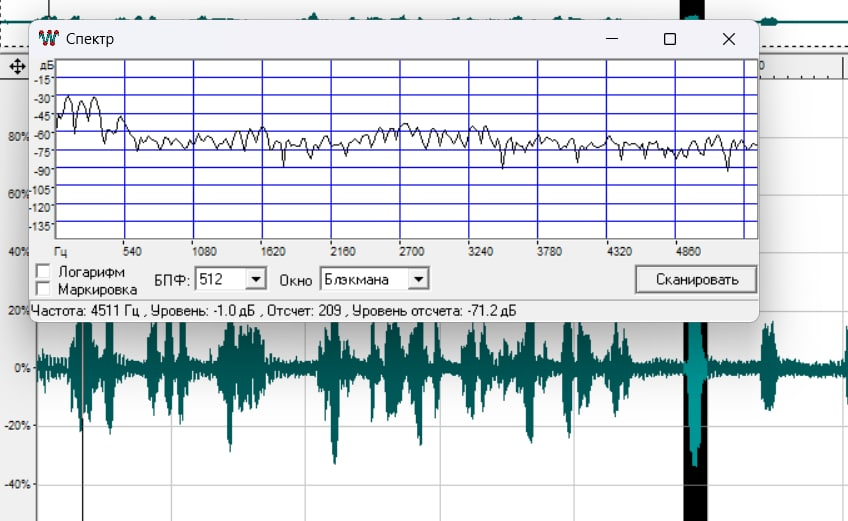
\includegraphics[scale=0.7]{inc/fig_09.jpg}
    \caption{Спектр гласного звука «А». БПФ 512, окно Блэкмана}
    \label{fig:fig09}
\end{figure}

\subsection*{Программа WaveView}

Необходимо отметить преимущество WaveView, которое заключается в возможности
выполнять полноценный вейвлет-анализ с последующим созданием
Вейвлет-сонограммы.

Так как человеческий голос является нестационарным сигналом, он не может быть
эффективным образом обработан средствами Фурье-анализа, использующего
разложение в сумму периодических функций. Ключевым свойством, которым обладает
Вейвлет-сонограмма и не обладает Фурье- спектрограмма, является локализация
особенностей сигнала, в том числе, низкочастотных.

В рамках анализа тестовой записи для звука «А» в программе WaveView построена
Вейвлет-сонограмма и частотное сечение. Определены частоты наиболее
энергетически сильных гармоник: первая гармоника соответствует частоте 127 Гц,
вторая – частоте 207 Гц. Результат показан на рисунке \ref{fig:fig10}.
При помощи возможностей WaveView по отображению временной позиции курсора было
определено время начала звука и время окончания, таким образом длительность
звука «А» составила 0,255 с.

\begin{figure}
    \centering
    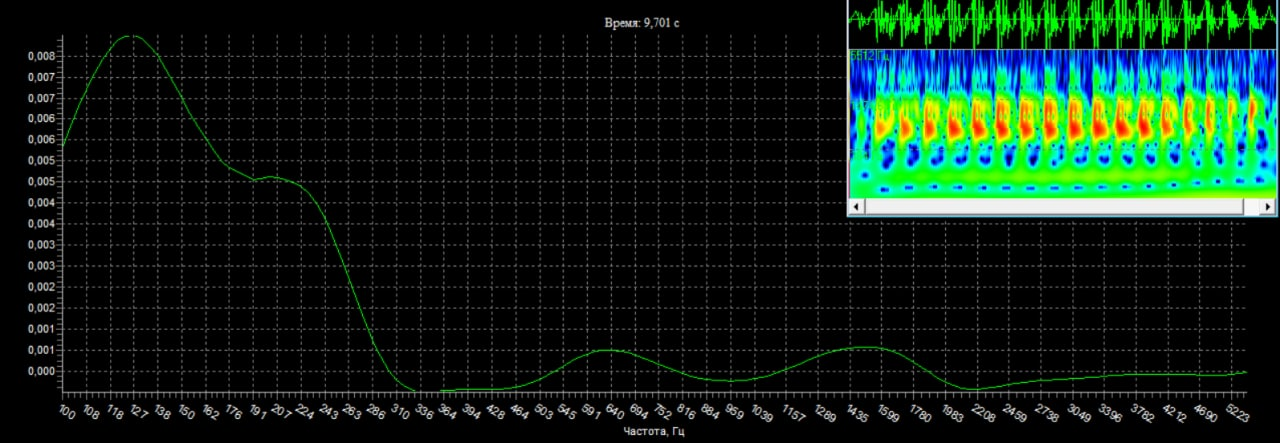
\includegraphics[scale=0.5]{inc/fig_10.jpg}
    \caption{
        Вейвлет-сонограмма гласного звука «А», сверху рисунка спектральное
        сечение выделенного участка сигнала 9,701 сек. Частота 1-й гармоники 127
        Гц, частота 2-й гармоники 207 Гц.
    }
    \label{fig:fig10}
\end{figure}

Аналогично для анализа согласных звуков был выбран звук был проанализирован
звук «В» в слове «двадцать», для него первая гармоника соответствует 88 Гц,
вторая – 170 Гц. Результат показан на рисунке \ref{fig:fig11}. Длительность
произнесения звука «В» на тестовой записи составляет 0,065 с.

\begin{figure}
    \centering
    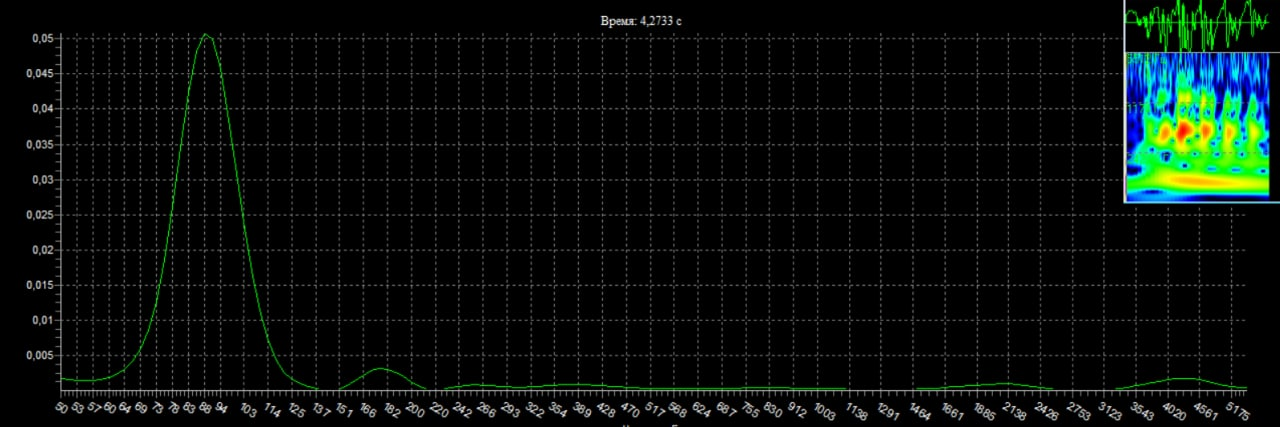
\includegraphics[scale=0.5]{inc/fig_11.jpg}
    \caption{
        Вейвлет-сонограмма согласного звука «В», сверху рисунка спектральное
        сечение выделенного участка сигнала 4,2733 сек. Частота 1-й гармоники
        88 Гц, частота 2-й гармоники 170 Гц.
    }
    \label{fig:fig11}
\end{figure}

Был проанализирован звук «Г» в слове «года», результат представлен на рисунке
\ref{fig:fig12}. Длительность произнесения звука на тестовой записи
составляет 0,102 с. Частота 1-й гармоники 114 Гц, частота 2-й гармоники 230 Гц.
Результат на рис. \ref{fig:fig12}.

\begin{figure}
    \centering
    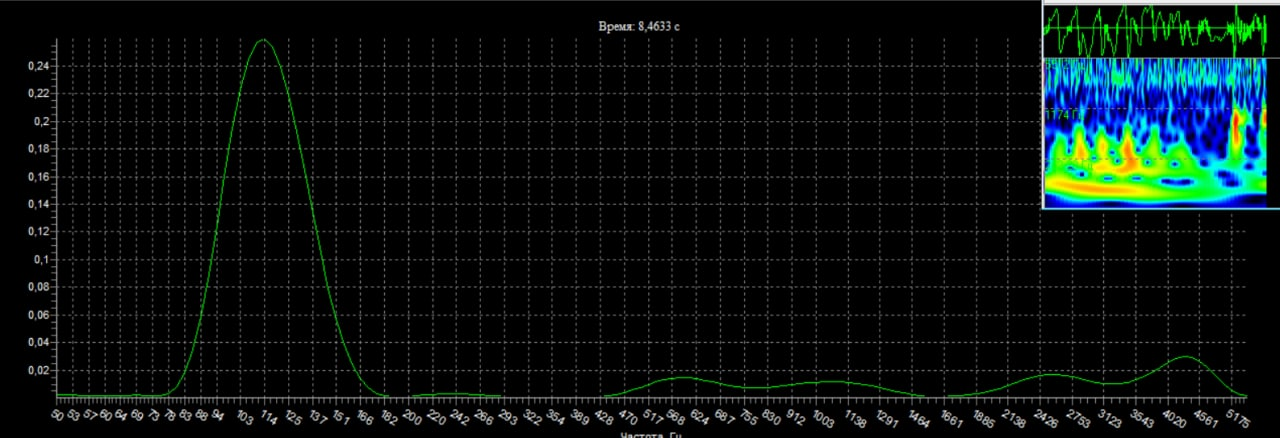
\includegraphics[scale=0.5]{inc/fig_12.jpg}
    \caption{
        Вейвлет-сонограмма согласного звука «Г», сверху рисунка спектральное
        сечение выделенного участка сигнала 8,4633 сек. Частота 1-й гармоники
        114 Гц, частота 2-й гармоники 230 Гц.
    }
    \label{fig:fig12}
\end{figure}
 % Практическая часть

    \conclusion

В ходе данного практического задания с использованием современных программных
средств были изучены:
\begin{enumerate}
    \item основные процедуры записи и обработки речевых сигналов;
    \item методы измерения параметров и анализа характеристик речевого сигнала,
          включая частотные характеристики гласных и согласных звуков.
\end{enumerate}

Определенные в рамках практической работы параметры звуков «А», «Б», «В»
приведены в таблице 4.

\begin{table}[ht]
\centering
\caption{Характеристики звуков}
\begin{tabular}{|c|c|cccc|}
\hline
\textbf{Звук} & \textbf{Слово-источник} & \multicolumn{4}{c|}{\textbf{Характеристики}} \\
\hline
             &                         & \textbf{Первая г.} & \textbf{Вторая г.} & \textbf{Длит.} & \textbf{Полоса частот} \\
\hline
А & А     & 127\,Гц   & 207\,Гц  & 0,255\,с   & 100--5223\,Гц \\
\hline
В & Двадцать & 88\,Гц   & 170\,Гц  & 0,065\,с  & 50--5175\,Гц \\
\hline
Г & Года & 114\,Гц   & 230\,Гц   & 0,102\,с  & 50--5175\,Гц \\
\hline
\end{tabular}
\end{table}

Рассмотрены возможности программных продуктов для работы со звуковыми сигналами
Praat, SoundEdit и WaveView. WaveView плохо работает на современных Windows и
обладает крайне плохим пользовательским интерфейсом, SoundEdit больше не
открывается на Windows 11. Хорошей альтернативой, по моему мнению, является
приложение с открытым исходным кодом Sonic Visualizer, поддерживающий систему
плагинов и обладающий большим комьюнити. Если какой-то возможности не хватает,
то лучше написать плагин в большую и хорошо работающую программу, чем
изобретать новую.
 % Заключение
    \structure{СПИСОК ЛИТЕРАТУРЫ}

    1. Горшков Ю.Г. Анализ и засекречивание речевого сигнала: Учебное пособие. М.: Издательство МГТУ им. Н.Э. Баумана. 2007. 34 с.

    2. Горшков Ю.Г. Криминалистическое исследование фонограмм / Методические указания к лабораторным работам. МГТУ им. Н.Э. Баумана. 2017. 32

    3. Горшков Ю.Г. Обработка речевых и акустических биомедицинских сигналов на основе вейвлетов / Научное издание. М.: Радиотехника. 2017. 240 с.

    4. P. Boersma and D. Weenink. Praat: Doing phonetics by computer (version 6.2.14) [computer program], 2022. (http://www.praat.org/)

    5. B. Hayes. Spectrogram reading practice, 2021. (https://linguistics. ucla.edu/people/hayes/103/SpectrogramReading/index.htm)

    6. Горшков Ю.Г. Визуализация многоуровневого вейвлет-анализа фонограмм //   Электронный журнал «Научная визуализация». Национальный Исследовательский   Ядерный Университет «МИФИ» № 2, том 7, квартал 2, 2015. C. 96-111.
 % Заключение
\end{document}
